\documentclass[mstat,12pt]{unswthesis}



%%%%%%%%%%%%%%%%%%%%%%%%%%%%%%%%%%%%%%%%%%%%%%%%%%%%%%%%%%%%%%%%%%
% 
% OK...Now we get to some actual input.  The first part sets up
% the title etc that will appear on the front page
%
%%%%%%%%%%%%%%%%%%%%%%%%%%%%%%%%%%%%%%%%%%%%%%%%%%%%%%%%%%%%%%%%%

\title{Capstone Project by Team Group 3\\[0.5cm]A Data Science Approach
to Forecast Electricity Consumption in NSW}

\authornameonly{John Student (z123456), Jim Student2 (zID), Rishantha
Rajakaruna (z5441528). }

\author{\Authornameonly}

\copyrightfalse
\figurespagefalse
\tablespagefalse

%%%%%%%%%%%%%%%%%%%%%%%%%%%%%%%%%%%%%%%%%%%%%%%%%%%%%%%%%%%%%%%%%
%
%  And now the document begins
%  The \beforepreface and \afterpreface commands puts the
%  contents page etc in
%
%%%%%%%%%%%%%%%%%%%%%%%%%%%%%%%%%%%%%%%%%%%%%%%%%%%%%%%%%%%%%%%%%%


\input{header.tex}

\usepackage{booktabs}
\usepackage[table,xcdraw]{xcolor}
\usepackage{colortbl}


\begin{document}

\beforepreface

%\afterpage{\blankpage}

% plagiarism

\prefacesection{Plagiarism statement}

\vskip 2pc \noindent I declare that this thesis is my
own work, except where acknowledged, and has not been submitted for
academic credit elsewhere. 

\vskip 2pc  \noindent I acknowledge that the assessor of this
thesis may, for the purpose of assessing it:
\begin{itemize}
\item Reproduce it and provide a copy to another member of the University; and/or,
\item Communicate a copy of it to a plagiarism checking service (which may then retain a copy of it on its database for the purpose of future plagiarism checking).
\end{itemize}

\vskip 2pc \noindent I certify that I have read and understood the University Rules in
respect of Student Academic Misconduct, and am aware of any potential plagiarism penalties which may 
apply.\vspace{24pt}

\vskip 2pc \noindent By signing 
this declaration I am
agreeing to the statements and conditions above.
\vskip 2pc \noindent
Signed: \rule{7cm}{0.25pt} \hfill Date: \rule{4cm}{0.25pt} \\[1cm]
Signed: \rule{7cm}{0.25pt} \hfill Date: \rule{4cm}{0.25pt} \\[1cm]
Signed: \rule{7cm}{0.25pt} \hfill Date: \rule{4cm}{0.25pt} \\[1cm]
\vskip 1pc

%\afterpage{\blankpage}

% Acknowledgements are optional


\prefacesection{Acknowledgements}

{\bigskip}TBW\ldots{}\\[1cm] 

{\bigskip\bigskip\bigskip\noindent} 25/07/2020.

%\afterpage{\blankpage}

% Abstract

\prefacesection{Abstract}

TBW \ldots{}

%\afterpage{\blankpage}


\afterpreface





%%%%%%%%%%%%%%%%%%%%%%%%%%%%%%%%%%%%%%%%%%%%%%%%%%%%%%%%%%%%%%%%%%
%
% Now we can start on the first chapter
% Within chapters we have sections, subsections and so forth
%
%%%%%%%%%%%%%%%%%%%%%%%%%%%%%%%%%%%%%%%%%%%%%%%%%%%%%%%%%%%%%%%%%%



%%%%%%%%%%%%%%%%%%%%%%%%%%%%%%%%%%%%%

%\afterpage{\blankpage}


\chapter{Introduction}\label{introduction}

Accurate Electricity demand forecasting is a fundamental component of
decision making for governments, regulatory bodies and businesses. To
forecast electricity demand we need to understand the drivers of demand
fluctuation and corresponding relationships. Weather changes, long-term
climate change and macroeconomic influences such as, population growth,
economic growth are key factors that influence demand \cite{a2024_nem}.
Additionally, generation of electricity through renewable sources such
as Solar and Wind which doubled over the last decade
\cite{energygovau_2024_renewables} has added more complexity to
forecasting due to its dependency on weather.

The demand forecasting varies from short term to medium and long term.
The parameters that influence each period type varies. Short term
forecasting focus on small time intervals. i.e.~few mins upto few days.
It can be heavily influenced by daily weather, time of the day and
holidays. In case of medium to long term forecast, the timeframe could
vary from few months to few years into the future and determined by long
term factors such as climate change, population growth, government
policy to name a few.

This research paper focus on short term forecasting. Therefore,
primarily use half hourly temperature, historical half hourly actual
demand, calendar information (holidays, weekends) and time of the day as
key data sources. We analyse in detail the relationship between demand
and the aforementioned features and use two models, \textbf{XGBoost} and
\textbf{Prophet by Facebook} to forecast daily demand.

By using multiple matrices, we compare the performance of each model.
Additionally, we also compare the results of the two models against the
short-term demand forecast published by Australian Energy Market
Operator.

We hope the findings will assist market participants to make informed
decisions with regards to short term electricity demand forecasting and
contribute to a more sustainable and efficient energy landscape.

\chapter{Literature Review}\label{literature-review}

Here are a few references that can be useful: \cite{Xie2018} and
\cite{Lafaye2013}. See also
\url{https://bookdown.org/yihui/rmarkdown-cookbook/}

\bigskip

In order to incorporate your own references in this report, we strongly
advise you use BibTeX. Your references then needs to be recorded in the
file \texttt{references.bib}.

\chapter{Material and Methods}\label{material-and-methods}

\section{Software}\label{software}

Primary software used for analysis and model build is Python. We have
used extensive set of python libraries. List of libraries used are,

\begin{itemize}
  \item holidays - Derive public holidays in NSW 
  \item pandas - Data selection and manipulation
  \item numpy - Calculations and data manipulation
  \item statsmodels - Used for statistical tests and statistical data exploration
  \item matplotlib, seaborn - To create plots and visualize statistical analysis
  \item scipy - statistical analysis
  \item sklearn - Model preparation and analysis
  \item xgboost - Used for XGBoost model build
  \item prophet - Used for Facebook Prophet model build
\end{itemize}

Jupyter Notebook and RStudio was used as integrated development
environments. Github repository was used for code management. Teams and
One Drive were used for collaboration and communication.

\section{Description of the Data}\label{description-of-the-data}

Following Data sets are used for this project.

\begin{enumerate}
    \item Total Electricity Demand NSW
    \item Air Temperature NSW
    \item NSW Calendar
    \item Total Forecast Demand NSW
\end{enumerate}

\subsection{Total Electricity Demand
NSW}\label{total-electricity-demand-nsw}

Total Electricity Demand in 30 min increments. This data is sourced from
the Market Management System database, which is published by the market
operator from the National Electricity Market (NEM) system.

\begin{table}[h]
\tiny
\begin{tabular}{@{}|l|l|l|l|@{}}
\toprule
\textbf{Row Count} & \textbf{File Size (Approx)} & \textbf{File Format} & \textbf{File Name}   \\ \midrule
196513             & 5.6 MB                      & CSV                  & totaldemand\_nsw.csv \\ \bottomrule
\end{tabular}
\end{table}

\begin{table}[h]
\tiny
\begin{tabular}{@{}|l|l|l|@{}}
\toprule
\rowcolor[HTML]{EFEFEF} 
\textbf{Attributes} & \textbf{Description}                                                                                             & \textbf{\begin{tabular}[c]{@{}l@{}}Attribute \\ Characteristics\end{tabular}} \\ \midrule
DATETIME            & \begin{tabular}[c]{@{}l@{}}Date and time interval of each observation. \\ Format (dd/mm/yyyy hh:mm)\end{tabular} & Timestamp                                                                     \\ \midrule
TOTALDEMAND         & Total demand in MW                                                                                               & Numeric                                                                       \\ \midrule
REGIONID            & Region Identifier (i.e. NSW1)                                                                                    & \begin{tabular}[c]{@{}l@{}}String.\\ Categorical\end{tabular}                 \\ \bottomrule
\end{tabular}
\end{table}

\subsection{\texorpdfstring{\emph{Air Temperature
NSW}}{Air Temperature NSW}}\label{air-temperature-nsw}

Air temperature in NSW (as measured from the Bankstown Airport weather
station). This data is sourced from the Australian Data Archive for
Meteorology. Note: Unlike the total demand and forecast demand, the time
interval between each observation may not be constant (i.e.~half-hourly
data). As noted in the literature review, temperature is a key driver of
demand. Therefore, this dataset is critically important for the research
question

\begin{table}[h]
\tiny
\begin{tabular}{@{}|l|l|l|l|@{}}
\toprule
\rowcolor[HTML]{EFEFEF} 
\textbf{Row Count} & \textbf{File Size (Approx)} & \textbf{File Format} & \textbf{File Name}   \\ \midrule
220326             & 6.7 MB                      & CSV                  & temperature\_nsw.csv \\ \bottomrule
\end{tabular}
\end{table}

\begin{table}[h]
\tiny
\begin{tabular}{@{}|l|l|l|@{}}
\toprule
\rowcolor[HTML]{EFEFEF} 
\textbf{Attributes} & \textbf{Description}                                                                                             & \textbf{\begin{tabular}[c]{@{}l@{}}Attribute \\ Characteristics\end{tabular}} \\ \midrule
DATETIME            & \begin{tabular}[c]{@{}l@{}}Date and time interval of each observation. \\ Format (dd/mm/yyyy hh:mm)\end{tabular} & Timestamp                                                                     \\ \midrule
TEMPERATURE         & Air temperature (°C)                                                                                             & Numeric                                                                       \\ \midrule
LOCATION            & \begin{tabular}[c]{@{}l@{}}Location of a weather station \\ (i.e., Bankstown weather station)\end{tabular}       & \begin{tabular}[c]{@{}l@{}}String\\ Categorical\end{tabular}                  \\ \bottomrule
\end{tabular}
\end{table}

\subsection{\texorpdfstring{\emph{NSW
Calendar}}{NSW Calendar}}\label{nsw-calendar}

Use NSW Calendar to include holidays, seasons, weekend information for
the model build

\begin{table}[h]
\tiny
\begin{tabular}{@{}|l|l|l|@{}}
\toprule
\rowcolor[HTML]{EFEFEF} 
\textbf{Attributes} & \textbf{Description}                                                                                                                                                                                         & \textbf{\begin{tabular}[c]{@{}l@{}}Attribute \\ Characteristics\end{tabular}} \\ \midrule
DATETIME            & \begin{tabular}[c]{@{}l@{}}Date and time interval of each observation. \\ Generated through Python library\end{tabular}                                                                                      & Timestamp                                                                     \\ \midrule
HOLIDAY             & \begin{tabular}[c]{@{}l@{}}Marked 1 if public holiday in NSW, otherwise 0. \\ Generated using 'holidays' Python library\\ Sourced from the python library \\ https://pypi.org/project/holidays/\end{tabular} & Numeric                                                                       \\ \midrule
SUMMER              & \begin{tabular}[c]{@{}l@{}}Marked 1 if the month \\ is in Summer season, else 0.\\ Use one hot encoding\end{tabular}                                                                                            & Numeric                                                                       \\ \midrule
AUTUMN              & \begin{tabular}[c]{@{}l@{}}Marked 1 if the month \\ is in Autumn season, else 0\\ Use one hot encoding\end{tabular}                                                                                             & Numeric                                                                       \\ \midrule
WINTER              & \begin{tabular}[c]{@{}l@{}}Marked 1 if the month \\ is in Winter season, else 0\\ Use one hot encoding\end{tabular}                                                                                             & Numeric                                                                       \\ \midrule
SPRING              & \begin{tabular}[c]{@{}l@{}}Marked 1 if the month \\ is in Spring season, else 0\\ Use one hot encoding\end{tabular}                                                                                             & Numeric                                                                       \\ \midrule
WEEKDAY             & \begin{tabular}[c]{@{}l@{}}Marked 1 if day of week is between \\ Monday to Friday, else 0\end{tabular}                                                                                                       & Numeric                                                                       \\ \midrule
DAYOFWEEK           & Marked 1 to 7 to indicate day of week                                                                                                                                                                        & Numeric                                                                       \\ \midrule
MONTH               & Month of the Year                                                                                                                                                                                            & Numeric                                                                       \\ \bottomrule
\end{tabular}
\end{table}

\subsection{\texorpdfstring{\emph{Total Forecast Demand
NSW}}{Total Forecast Demand NSW}}\label{total-forecast-demand-nsw}

Forecast demand in half-hourly increments for NSW. Data also sourced
from the Market Management System database. This dataset would be
valuable for us to validate the outcome of our model. Especially to
understand the accuracy.

\begin{table}[h]
\tiny
\begin{tabular}{@{}|l|l|l|l|@{}}
\toprule
\rowcolor[HTML]{EFEFEF} 
\textbf{Row Count} & \textbf{File Size (Approx)} & \textbf{File Format} & \textbf{File Name}      \\ \midrule
10906019           & 722 MB                      & CSV                  & forecastdemand\_nsw.csv \\ \bottomrule
\end{tabular}
\end{table}

\begin{table}[h]
\tiny
\begin{tabular}{@{}|l|l|l|@{}}
\toprule
\rowcolor[HTML]{EFEFEF} 
\textbf{Attributes} & \textbf{Description}                                                                                                                                                                                                                                                              & \textbf{\begin{tabular}[c]{@{}l@{}}Attribute \\ Characteristics\end{tabular}} \\ \midrule
DATETIME            & \begin{tabular}[c]{@{}l@{}}Date and time interval of each observation. \\ Format (dd/mm/yyyy hh:mm)\end{tabular}                                                                                                                                                                  & Timestamp                                                                     \\ \midrule
FORECASTDEMAND      & Forecast demand in MW                                                                                                                                                                                                                                                             & Numeric                                                                       \\ \midrule
REGIONID            & Region Identifier (i.e. NSW1)                                                                                                                                                                                                                                                     & \begin{tabular}[c]{@{}l@{}}String\\ Categorical\end{tabular}                  \\ \midrule
PREDISTPATCHSEQNO   & \begin{tabular}[c]{@{}l@{}}Unique identifier of predispatch run (YYYYMMDDPP). \\ In energy generation, “dispatch” refers to process of \\ sending out energy to the power grid to meet energy demand. \\ “Predispatch” then is an estimated forecast of this amount.\end{tabular} & \begin{tabular}[c]{@{}l@{}}String \\ (Identifier)\end{tabular}                \\ \midrule
PERIODID            & Period count, starting from 1 for each predispatch run.                                                                                                                                                                                                                           & \begin{tabular}[c]{@{}l@{}}Numeric \\ (Identifier)\end{tabular}               \\ \midrule
LASTCHANGE          & \begin{tabular}[c]{@{}l@{}}Date time interval of each update of the \\ observation (dd/mm/yyyy hh:mm)\end{tabular}                                                                                                                                                                & Timestamp                                                                     \\ \bottomrule
\end{tabular}
\end{table}

\section{Pre-processing Steps}\label{pre-processing-steps}

\subsection{Merge and read zip files}\label{merge-and-read-zip-files}

All of the data files (excluding NSW Calendar) were stored in zip files.
Instead of exacting the the content of the files, we read directly the
zip file content for data cleaning. Only exception was the forecast
demand dataset where it was split to two zip files. Therefore these
files had to be merged as one zip prior to consumption.

\section{Data Cleaning}\label{data-cleaning}

Following activities were done as part of data cleaning.

\begin{itemize}
  \item Verify the data types, no of rows/columns and measure of central tendency.
  \item Removal of unused columns. 
    \begin{itemize}
      \item Total Electricity Demand NSW - 'REGIONID' was removed as this attribute had only one value and was not useful.
      \item Air Temperature NSW - 'LOCATION' was removed as this attribute had only one value and was not useful.
    \end{itemize}
  \item Verify whether NULL values exist. None found in the files.
  \item Validate whether duplicate rows exist
    \begin{itemize}
      \item Total Electricity Demand NSW - None found
      \item Air Temperature NSW - 13 duplicate rows were removed
    \end{itemize}
  \item Verify whether data is missing by validating that all the dates are available between the minimum and maximum dates in the file
    \begin{itemize}
      \item Total Electricity Demand NSW - None found
      \item Air Temperature NSW - Data for three dates were missing. 2016-07-16 till 2016-07-18. No action was taken as its a small percentage and also data is too far in the past and was not relevant for our research question.
    \end{itemize}
  \item Validate whether demand is recorded consistently for each day. 
    \begin{itemize}
      \item Total Electricity Demand NSW - It was noted that for 2021, there were only 2 months of data. Also for month of March, there was only one row. Therefore this had to be removed to ensure consistency.
      \item Air Temperature NSW - Temperature readings were not restricted to 30min intervals.Therefore we verified whether a temperature reading exist for every 30min. Where temperature readings were missing, we used fill forward method to add missing values. No of readings missing were 579 which is a small percentage.
    \end{itemize}
  \item Generate Calendar Data set. Python library \textit{holidays} was used to identify NSW holidays. Combining a date range and the holiday dates, we created a new calender dataset. Calender was limited to the date range of demand and temperature dataset.Additional attributes such as season (spring, summer, etc), day of week, weekday were derived.
    
\end{itemize}

Final dataset was prepared after completing the above activities. This
dataset was stored as a separate csv file for further consumption. It
should be noted that additional attributes `HOUR' and `PEAK' were also
included. Here `PEAK' is defined as `1' when the Time of the day is
between 7:00 AM and 10:00 PM. The time period for peak was derived from
\url{https://www.canstarblue.com.au/electricity/peak-off-peak-electricity-times/}.

\section{Assumptions}\label{assumptions}

The temperature data is limited to one location. Bankstown Airport.
However the electricity demand is measured for the entire state. As we
know, the temperature varies across different locations within the
state. Therefore we make an assumption that temperature at a single
point is sufficient for demand forecast for the entire state.

Popularity of rooftop solar has increased over the years whilst
manufacturing landscape has changed (as noted in literature review). The
impact of these factors are not part of the analysis due to lack of
publicly available data.

\section{Modelling Methods}\label{modelling-methods}

As per our initial research combined with literature review and
considering the time constraints, we will focus on two models for this
project. An additive model \textbf{Prophet} by \textbf{Facebook} and
another popular short term demand forecasting machine learning model
\textbf{XGBoost}. These two models will be tested across various
features such as temperature, hour of the day, holiday/non-holiday,
weekdays/weekends and peak/off-peak period.

Since the research question relates to short term demand, we intend to
use the latest available data instead of past data. Therefore the
dataset would be restricted to 3 years. We would also use 80:20 split of
data for training and testing. In relation to hyper-parameter tuning,
based on the model either random or grid search would be used.

\chapter{Exploratory Data Analysis}\label{exploratory-data-analysis}

Lets begin by analyzing the data to understand its characteristics.

\section{Yearly Electricity Demand}\label{yearly-electricity-demand}

Analysis of the electricity demand over the years would help identify
historic trends and any seasonal effects. As a start, lets review
average, Minimum and Maximum demand fluctuation over the years.

\begin{center}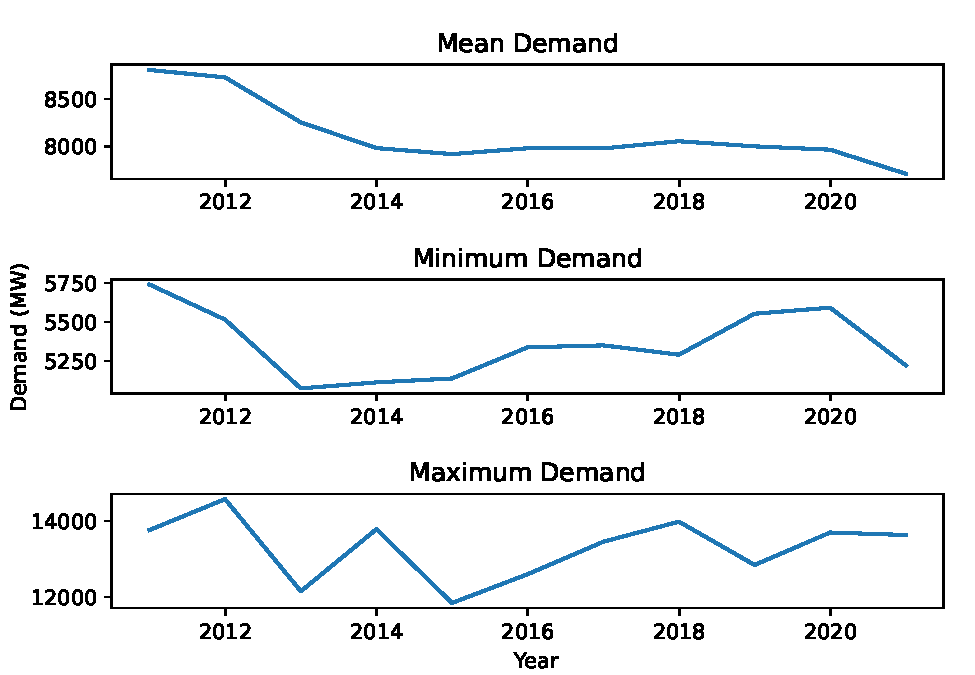
\includegraphics[width=0.5\linewidth]{unsw-ZZSC9020-report-template_files/figure-latex/unnamed-chunk-2-1} \end{center}

It is evident that the the average demand has reduced or flat lined over
the years. We were expecting the demand to rise with the population
growth over the years. Therefore, it would be prudent use latest
available data for model build as we are focusing on short term demand.

The minimum and maximum demand seem to fluctuate within a range and does
not indicate any significant trends.

\textit{Note: A potential reason for decrease in demand could be the increase use of roof top solar panels. Below graph from Australian PV Institute \url{https://pv-map.apvi.org.au/analyses} shows a clear increase in Solar panel installation. However further research is required to confirm any relationship.}

\begin{figure}[!h]
  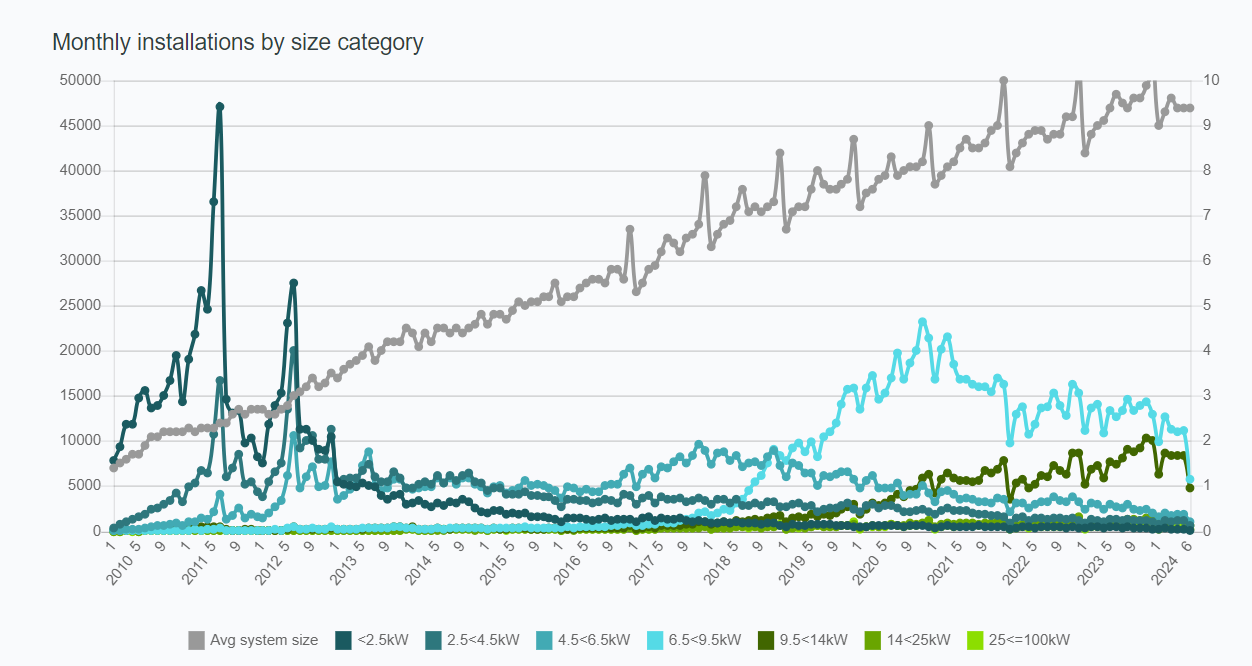
\includegraphics[width=0.4\linewidth]{AusPVInst.PNG}
  \caption{Yearly Solar PV Installation}
  \label{fig:Solar PV Installation }
\end{figure}

\section{Decompose Time series}\label{decompose-time-series}

Electricity demand data is of time series nature. According to
Australian Energy market operator (AEMO), Time series models are more
applicable in short-term forecasting \cite{aemo2023forecasting} similar
to our research question. Time series data can be decomposed to four
components. \cite{brownlee_2017_how}

\begin{itemize}
  \item Level - The average value in the series.
  \item Trend - The increasing or decreasing value in the series.
  \item Seasonality - The repeating short-term cycle in the series.
  \item Noise - The random variation in the series.
\end{itemize}

\begin{center}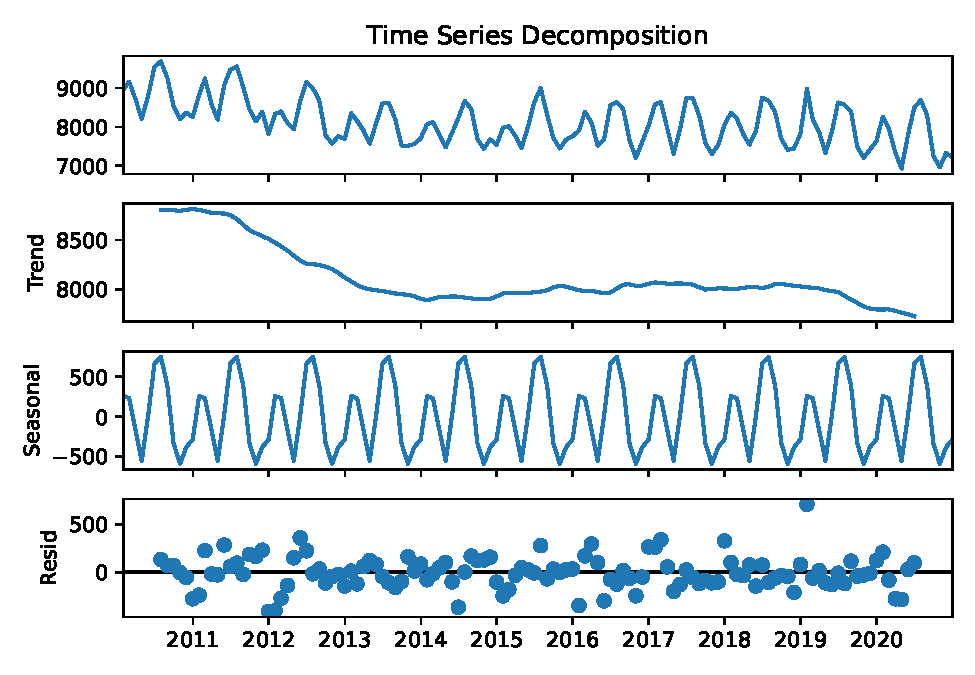
\includegraphics[width=0.5\linewidth]{unsw-ZZSC9020-report-template_files/figure-latex/unnamed-chunk-3-3} \end{center}

The Level and Trend plots both show gradual decline in demand similar to
what we observed earlier. The seasonal plot shows the peaks and troughs
in a repetitive pattern. This maybe due to relative high usage of
electricity during Winter (for heating) and Summer (for cooling)
compared to Spring and Autumn.

Further, to verify that the data set used is suitable for time series
analysis we perform a stationarity test using ADF (Augmented
Dickey-Fuller).

The null(H0) and alternate hypothesis(H1) of ADF test are:

\begin{itemize}
  \item H0: The series has a unit root (value of a=1),the series is non-stationary.
  \item H1: The series has no unit root, the series is stationary.
\end{itemize}

If we cannot reject the null hypothesis, we can say that the series is
not stationary, and if we do, it is considered stationary.

\begin{verbatim}
## Results of Dickey-Fuller Test:
\end{verbatim}

\begin{verbatim}
## Test Statistic                   -5.586991
## p-value                           0.000001
## #Lags Used                       28.000000
## Number of Observations Used    3989.000000
## Critical Value (1%)              -3.431990
## Critical Value (5%)              -2.862265
## Critical Value (10%)             -2.567156
## dtype: float64
\end{verbatim}

Based on the results we can observe that the test statistic is lower
than the critical values. Therefore we can reject the null hypothesis
and conclude that the time series is stationary.

\section{Monthly Demand}\label{monthly-demand}

Lets analyse the impact of demand based on the month.

\begin{center}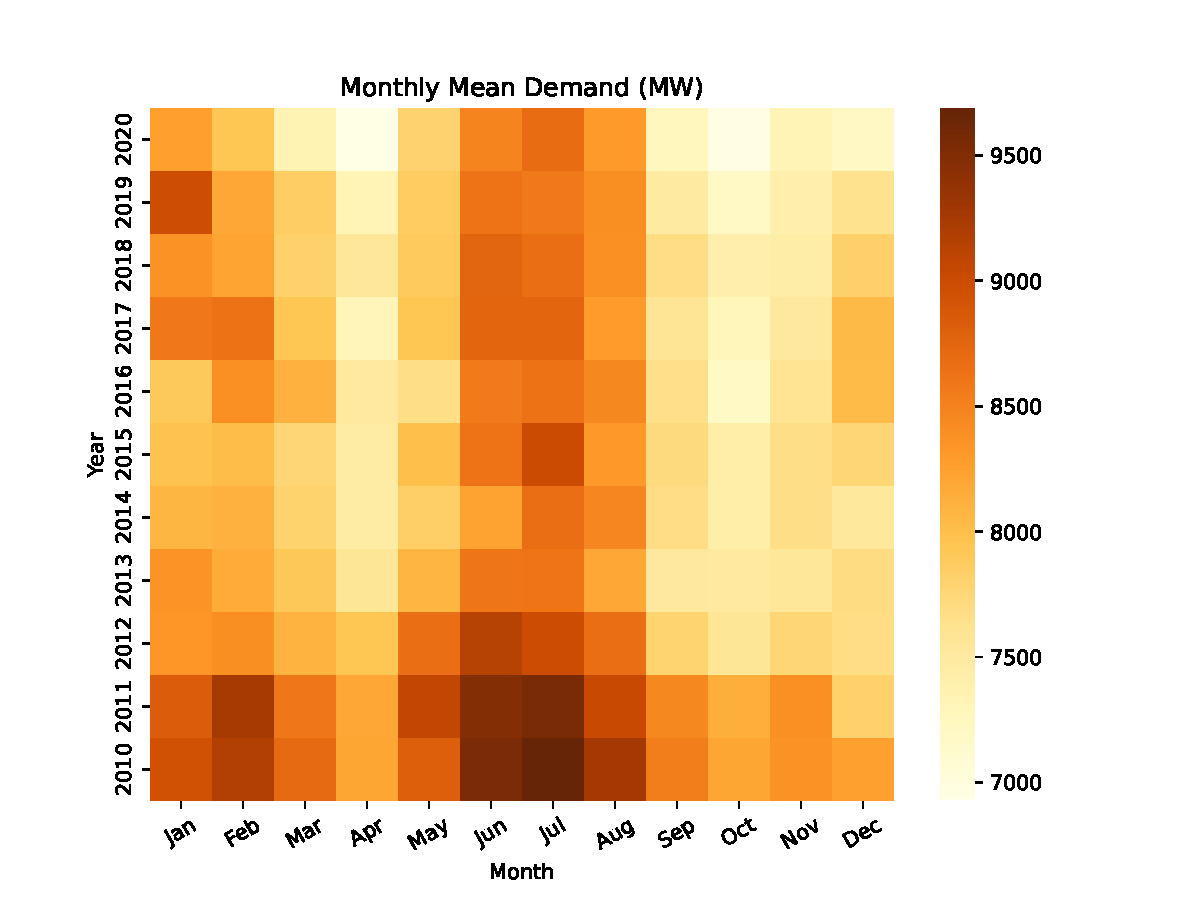
\includegraphics[width=0.5\linewidth]{unsw-ZZSC9020-report-template_files/figure-latex/unnamed-chunk-5-5} \end{center}

We tend to use heating during winter months and cooling during summer.
The heatmap clearly indicates that June, July, August winter months and
January, February Summer months have a higher average demand for
electricity. Conversely Spring and Autumn has a lower average demand.
Therefore the month/season should be considered for the model build.

\section{Day of the week Demand}\label{day-of-the-week-demand}

Next we analyse whether the electricity demand fluctuate depending on
the day of the week. As per the heatmap, weekends tend to have lower
demand. This could be due to the fact that most offices, factories are
closed during the weekend. Also, many people tend to spend weekends
outside. Similar to month, day of the week seems to have an influence on
the demand. Hence suitable to be included in the model build.

\begin{center}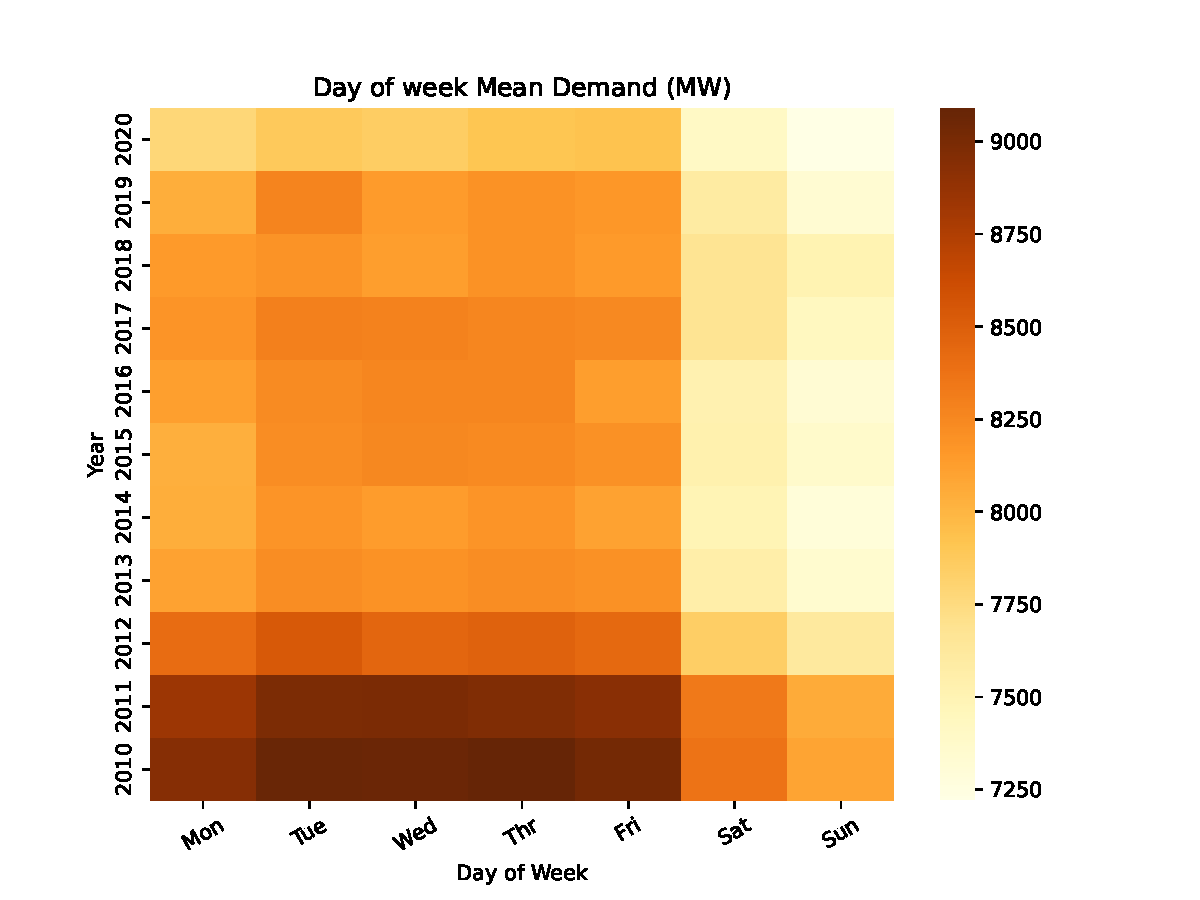
\includegraphics[width=0.5\linewidth]{unsw-ZZSC9020-report-template_files/figure-latex/unnamed-chunk-6-7} \end{center}

\section{Demand on Holidays}\label{demand-on-holidays}

Extending on the day of the week demand, we would like to analyse the
difference in average demand between holidays and non-holidays. For the
purpose of the analysis, we consider Public holidays and weekends as
\textit{Holidays} and all the other days as non-holidays.

\begin{center}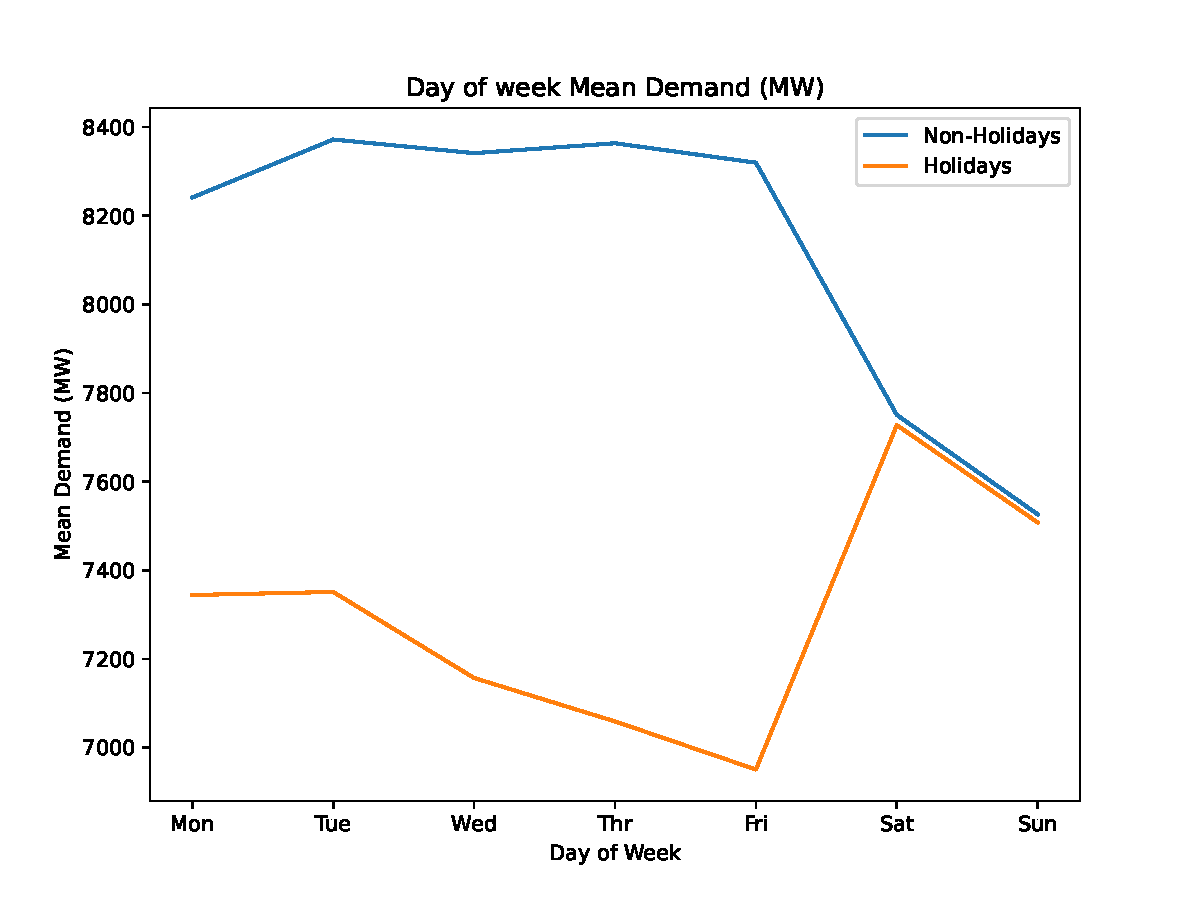
\includegraphics[width=0.5\linewidth]{unsw-ZZSC9020-report-template_files/figure-latex/unnamed-chunk-7-9} \end{center}

The graph clearly indicate a significant difference in mean demand
between holidays and non-holidays. As noted previously for Saturday and
Sunday, this may be due the fact that offices, factories not operating
over holidays resulting in lower demand. Therefore we could conclude
that holidays has a impact on the overall demand and therefore should be
considered in the model.

\section{Hour of the day demand}\label{hour-of-the-day-demand}

At the next granular level, we would like to observe how demand
fluctuates within a day (hour by hour). Australian energy providers
broadly segregates hourly demand to three groups
\cite{wrigley_2019_peak}. Peak, off-peak and shoulder. There are
variations of this by providers. For our analysis purposes, we would
simplify to Peak and Off-peak only.

\begin{center}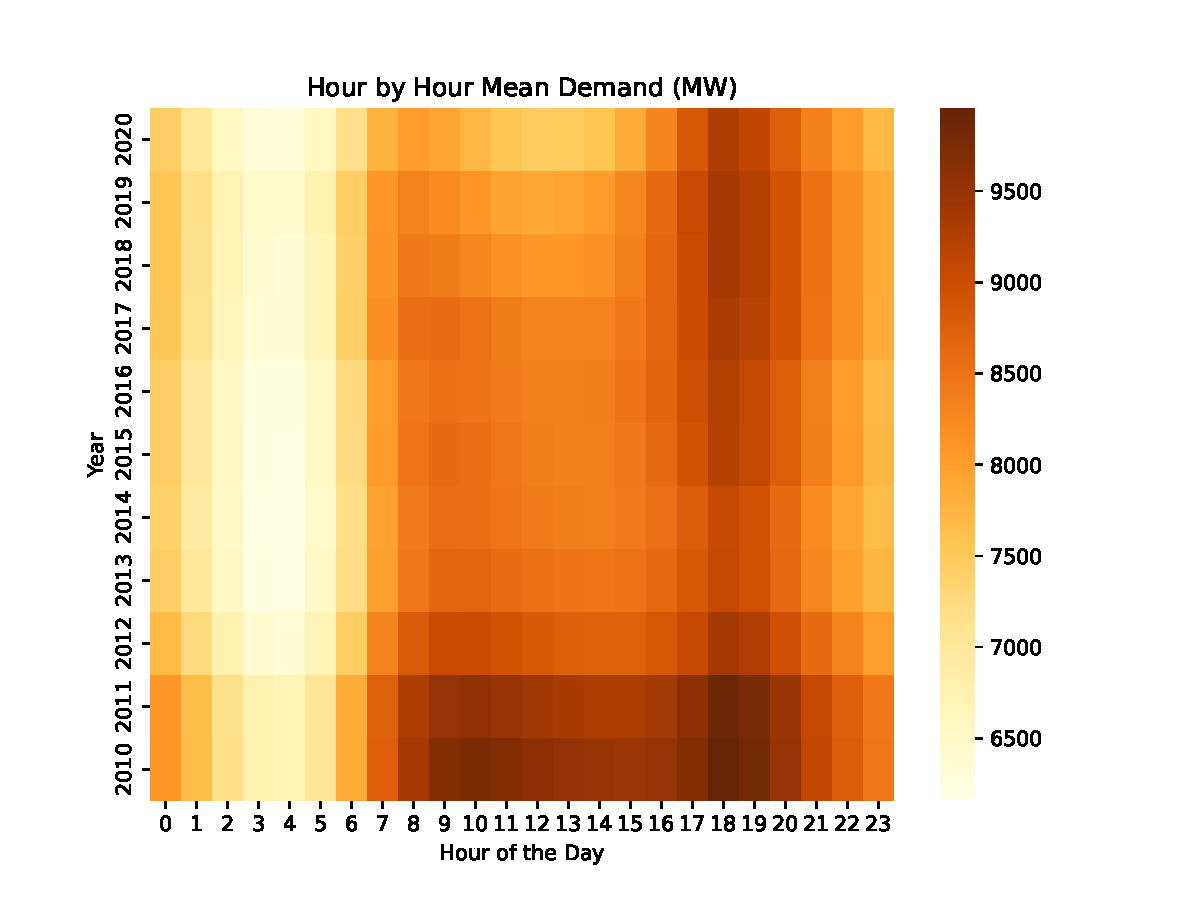
\includegraphics[width=0.5\linewidth]{unsw-ZZSC9020-report-template_files/figure-latex/unnamed-chunk-8-11} \end{center}

As evident from the graph, approx from 7:00 AM to 10:00 PM, the demand
seems to be high. Therefore we would use that period as Peak demand and
rest as off-peak demand for our model build.

\section{Peak vs Off-Peak demand}\label{peak-vs-off-peak-demand}

Based on previous analysis, lets verify the variations in demand based
on Peak hours vs off-peak. Additionally, we further drill-down on
holidays vs non-holidays.

\begin{center}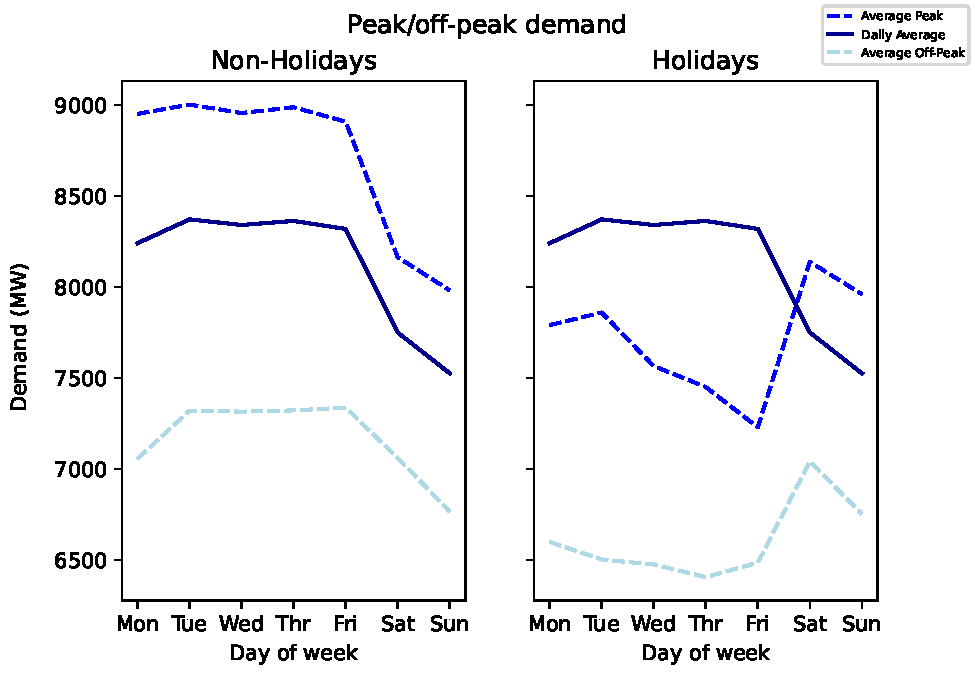
\includegraphics[width=0.75\linewidth]{unsw-ZZSC9020-report-template_files/figure-latex/unnamed-chunk-9-13} \end{center}

The graphs clearly indicate the difference in demand between peak and
off-peak hours. This pattern is visible both during non-holidays and
holidays. Therefore we should consider Peak/Off-Peak demand in the model
build.

\section{Autocorrelation \& Lag}\label{autocorrelation-lag}

We would like to understand the influence of Lag in the chosen model.
Prior to that lets review the concept.

Autocorrelation (serial correlation) is correlation between two values
of the same variable at times \(t\) and \(t_k\). When a value from a
time series is regressed on previous values from that same time series,
it is referred to as an autoregressive model. e.g \(y_t\) and
\(y_{t-1}\) \[ y_t = \beta_0 + \beta_1 y_{t-1} + \epsilon_t\] The above
is a first order autoregressive model. Meaning only one proceeding value
is used as predictor variable and is written as AR(1). If we used two
previous values as predictors, then it would be a second order
autoregressive model i.e.~AR(2). This can be generalised as AR(k), i.e
\(k^{th}\) order autoregressive model
\cite{thepennsylvaniastateuniversity_102}.

The autocorrelation function (ACF) is given as,
\(Corr(y_t,y_{t-k}),k=1,2,..n\) \cite{nist_2020_13512} where k is the
time gap or the lag between values of the same variable. We are
interested in Partial Autocorrelation, which measure the association
between \(y_t\) and \(y_{t-k}\) directly and filter out the linear
influence of the random variables that lie in between. PACF is useful to
identify the order of autocorrelation.

\begin{center}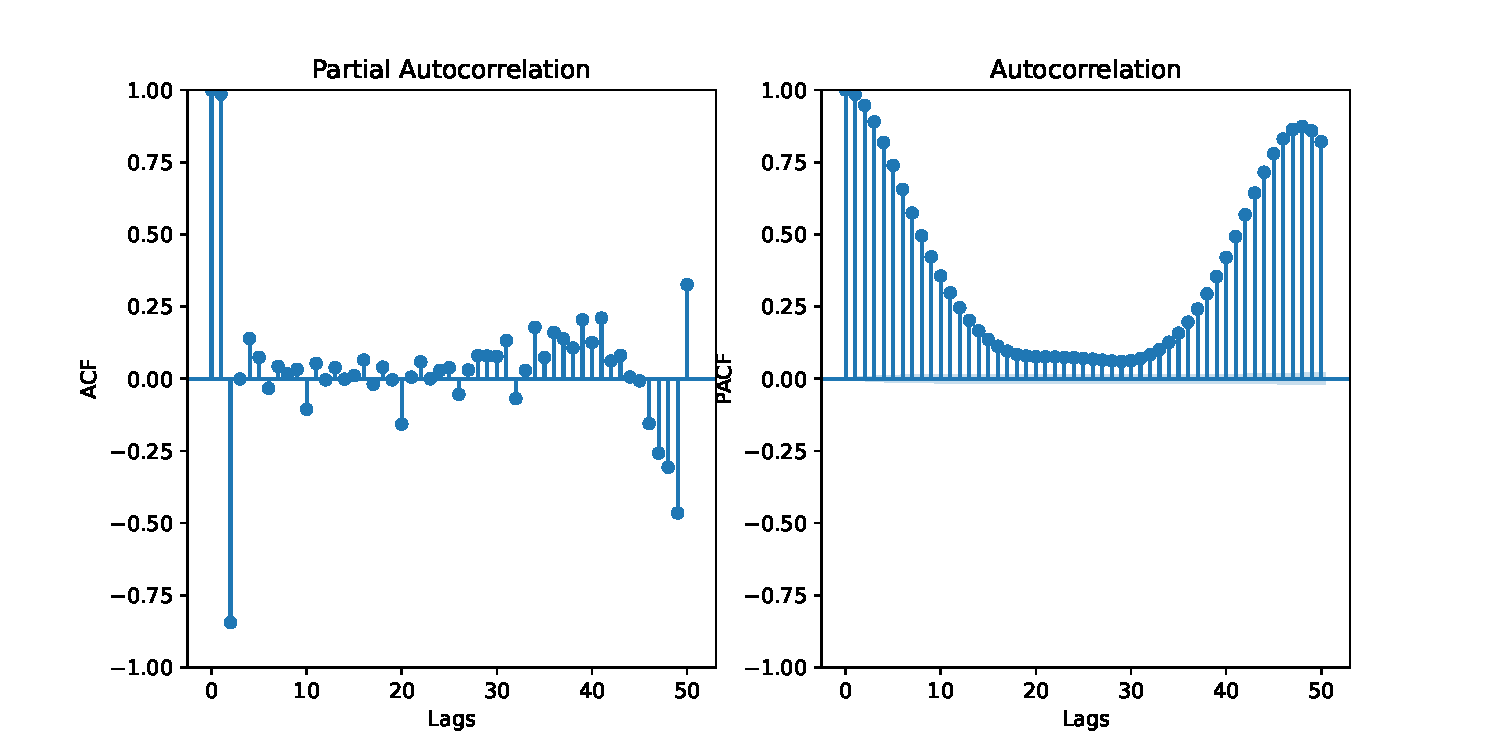
\includegraphics[width=0.7\linewidth]{unsw-ZZSC9020-report-template_files/figure-latex/unnamed-chunk-10-15} \end{center}

The ACF plot seems to indicate cyclical pattern and this could be due to
seasonality effect on the demand data. It also seem to highlight high
correlation between adjacent data points.

The PACF graph shows significant spike in lag 1,2 and 3 but seems to
decay as it moves along. Hence it maybe useful to limit to 3 lags for
the model.

\section{Temperature and demand
relationship}\label{temperature-and-demand-relationship}

The relationship between temperature and electricity demand is well
known. In below grpah, as the temperature increase, it is clearly
evident that demand increases. However it is interesting to note that
when temperature decreases, especially below 10 degrees, we see a
limited spike in demand. Potential reason could be that in NSW
temperature falls mostly during the night / early morning and therefore
consumers do not necessarily need heating. However the high temperatures
are mostly during day time and as a result people use electricity for
cooling driving up the demand.

\begin{center}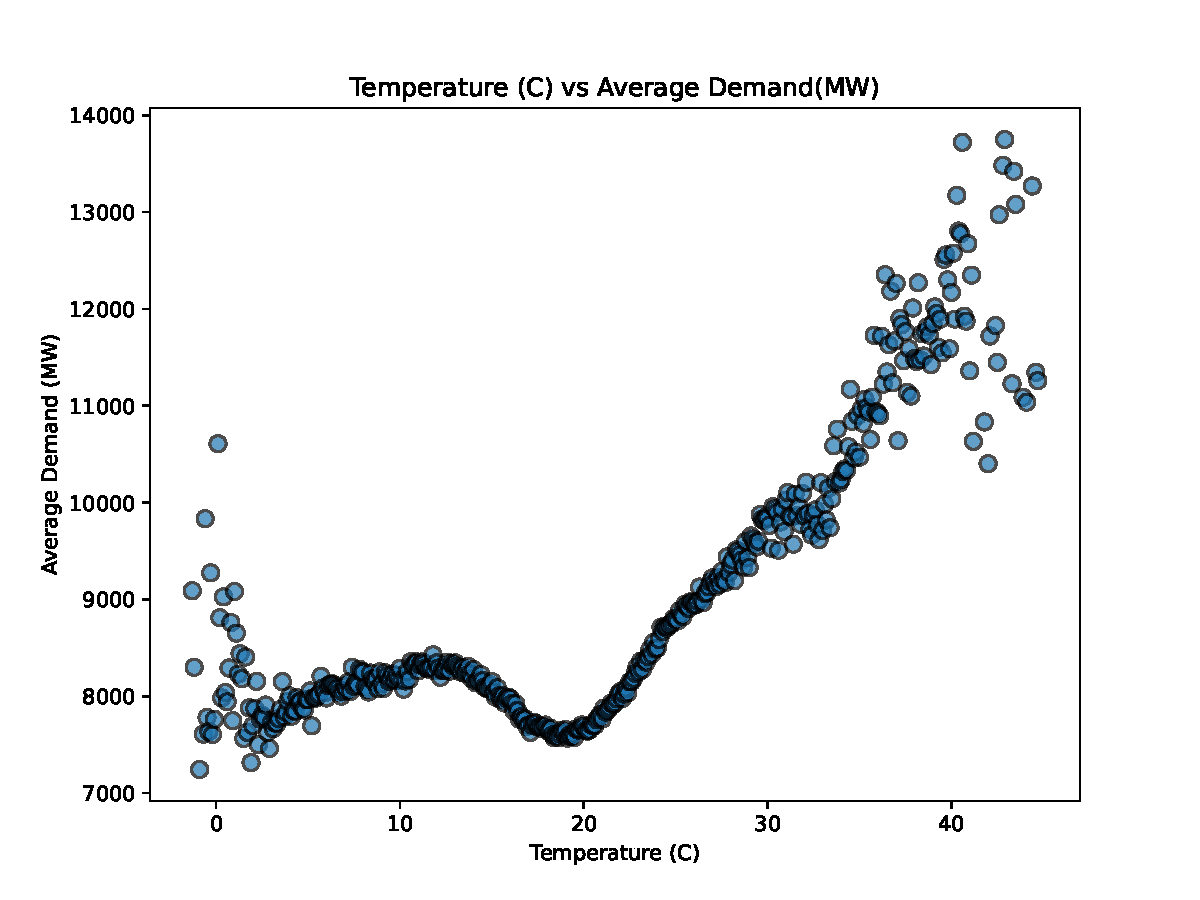
\includegraphics[width=0.5\linewidth]{unsw-ZZSC9020-report-template_files/figure-latex/unnamed-chunk-11-17} \end{center}

\section{Correlation matrix}\label{correlation-matrix}

Finally we look at the correlation between the attributes. The graph
below shows very low correlation between Total Demand and Temperature
this due the the fact that the relationship is non linear. Similarly,
Holiday and Month seems to have little or no correlation with respect to
demand. Hour and Peak/off-peak in turn seems to have higher correlation.

\begin{center}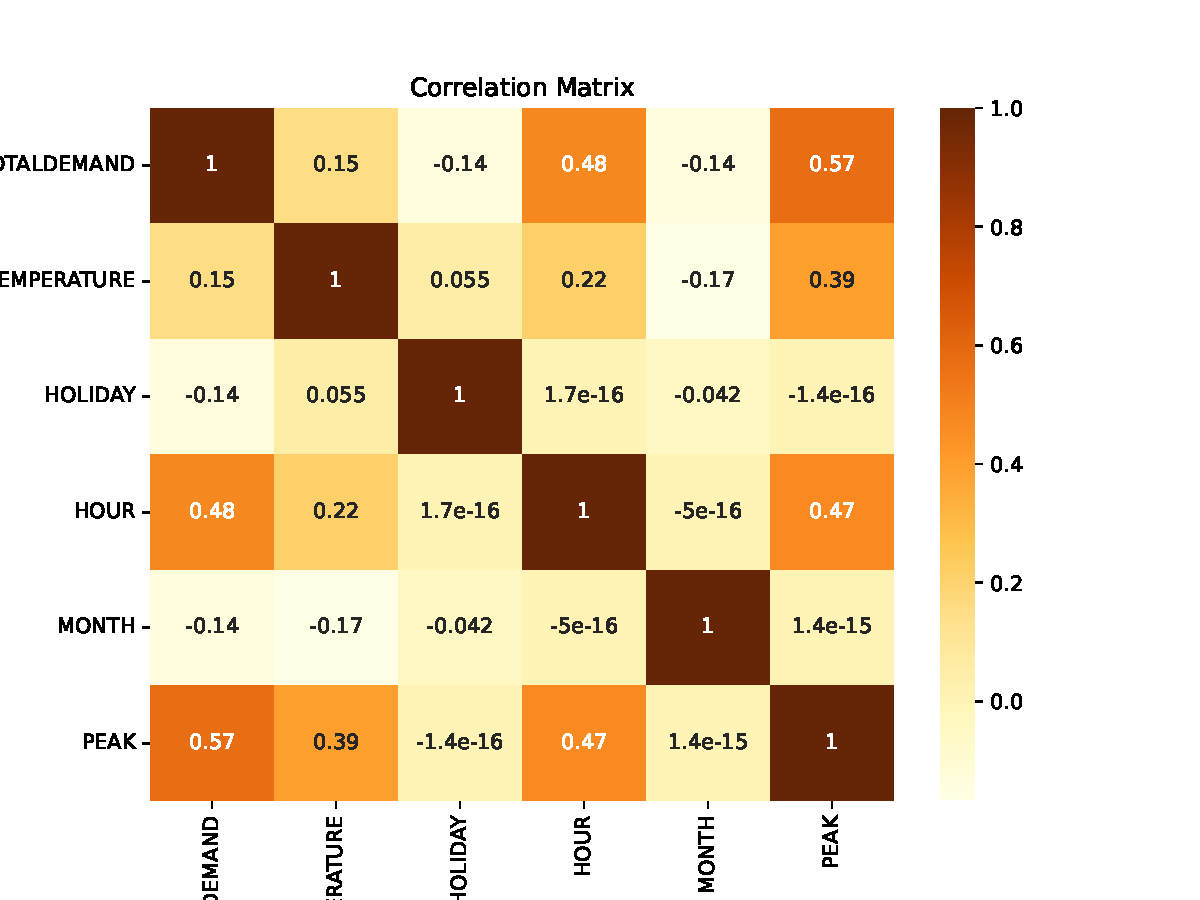
\includegraphics[width=0.5\linewidth]{unsw-ZZSC9020-report-template_files/figure-latex/unnamed-chunk-12-19} \end{center}

\section{Covid impact on Demand}\label{covid-impact-on-demand}

Since the dataset used overlaps with the Covid period, it is important
to understand if there is any impact on overall demand.

\begin{center}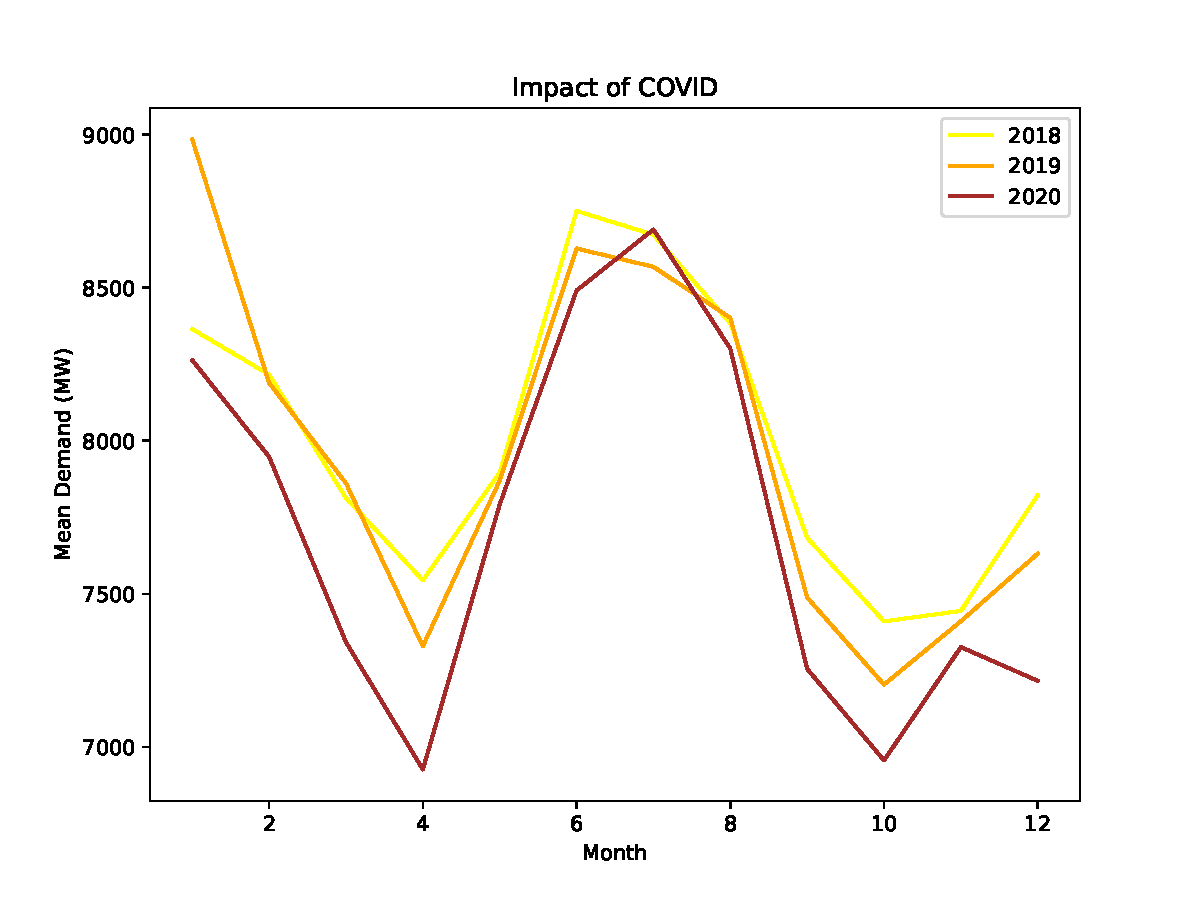
\includegraphics[width=0.5\linewidth]{unsw-ZZSC9020-report-template_files/figure-latex/unnamed-chunk-13-21} \end{center}

The plot does not indicate any significant deviations in the demand. One
could conclude that 2020 covid period had minimal impact on overall
demand based on the graph. However, further research is warranted to
confirm the finding.

\chapter{Analysis and Results}\label{analysis-and-results}

\section{A First Model}\label{a-first-model}

Having a very simple model is always good so that you can benchmark any
result you would obtain with a more elaborate model.

\bigskip

For example, one can use the linear regression model

\[
Y_i = \beta_0 + \beta_1 x_{1i} + \cdots \beta_p x_{pi} + \epsilon_i, \qquad i=1,\ldots,n.
\] where it is assumed that the \(\epsilon_i\)'s are i.i.d.~\(N(0,1)\).

\chapter{Discussion}\label{discussion}

Put the results you got in the previous chapter in perspective with
respect to the problem studied.

\chapter{Conclusion and Further
Issues}\label{conclusion-and-further-issues}

What are the main conclusions? What are your recommendations for the
``client''? What further analysis could be done in the future?

A figure:

\begin{figure}[H]
\includegraphics{unsw-logo.png}
\caption{A caption}\label{myfigure}
\end{figure}

In the text, see Figure \ref{myfigure}.

\bibliographystyle{elsarticle-harv}
\bibliography{references}

\chapter*{Appendix}\label{appendix}
\addcontentsline{toc}{chapter}{Appendix}

\section*{\texorpdfstring{\textbf{Codes}}{Codes}}\label{codes}
\addcontentsline{toc}{section}{\textbf{Codes}}

Add you codes here.

\section*{\texorpdfstring{\textbf{Tables}}{Tables}}\label{tables}
\addcontentsline{toc}{section}{\textbf{Tables}}

If you have tables, you can add them here.

Use \url{https://www.tablesgenerator.com/markdown_tables} to crete very
simple markdown tables, otherwise use \LaTeX.

\begin{longtable}[]{@{}lcr@{}}
\toprule\noalign{}
Tables & Are & Cool \\
\midrule\noalign{}
\endhead
\bottomrule\noalign{}
\endlastfoot
col 1 is & left-aligned & \$1600 \\
col 2 is & centered & \$12 \\
col 3 is & right-aligned & \$1 \\
\end{longtable}







\end{document}

